

\chapter{設計と実装}
\label{chap:system}
本章では「Web上の文章を成形すること」の定義を明確にした上で、
その実装形態である「ReaderLint」の要件と設計について述べる。

\section{システムの定義}
第一章にて示した文章の成形問題を解決するための要件は以下の4つであると仮定し、設計を行なった。

\begin{enumerate}
	\item 文章のリーダビリティの研究に基づき、読み手側のデバイスに向上させる改行を行う。
	\item 書き手側がつけた改行が文章の段落位置が読み手側から見たときに可読性を損ねていた場合には操作を行う。
	\item 文章内のリンク、emojiといった装飾を破壊しない。
	\item 1, 2, 3 を踏まえた上で書き手側の意図(改行による段落生成など)、書き手側の文意を損ねることなく行う
\end{enumerate}
上記の四つの要件を踏まえた上でシステムの実装を記す。

\newpage

\section{ReaderLintの機能}
ReaderLintはブラウザ上にレンダリングされている文章に対し、文章の折り返し地点にて文節を跨がった状態であった場合、
その文節前に改行処理を加えることで文節ごとの改行レイアウトを実現するというサービスである。処理をかける文章はデバイス内の
DOMにレンダリングされた文章なのでその表示環境に応じた改行レイアウト処理を行うことができる。
また、2.2.1 Web 上の文章の特色 にて提示した句点代わりに行われる改行を用いたレイアウトだった場合、読み手側ので表示される文章レイアウトにて
視認性を大きく損ねていないと判定された場合は改行を再度行い、違和感を緩和する機能を入れている。

\section{基本構成}

本システムはGoogle社の提供するブラウザであるChrome拡張機能としてJavaScript製で実装されている。
Chromeには個々ユーザーに対して公開されている、もしくは自作のJavaScript製のコードをインストールすることで
拡張機能としてブラウザ内で使用することができる。
ReaderLintもこのChormeの拡張機能としてインストールを行うことで使用可能である。

ReaderLintのインストール後には左クリックでコンテキストメニュー上に表示され、
メニューをクリックするとReaderLintを実行するDOMを選択できる状態になる。
この状態でテキストが挿入されているDOMをクリックすると指定したDOM内のHTML要素からテキスト箇所の
解析を行い、処理を行なったテキストを反映する。上記の処理をサーバーを用いずにクライアントサイドのみで
稼働する実装となっている。

\begin{figure}[H]
    \centering
    \label{fig:image9}
    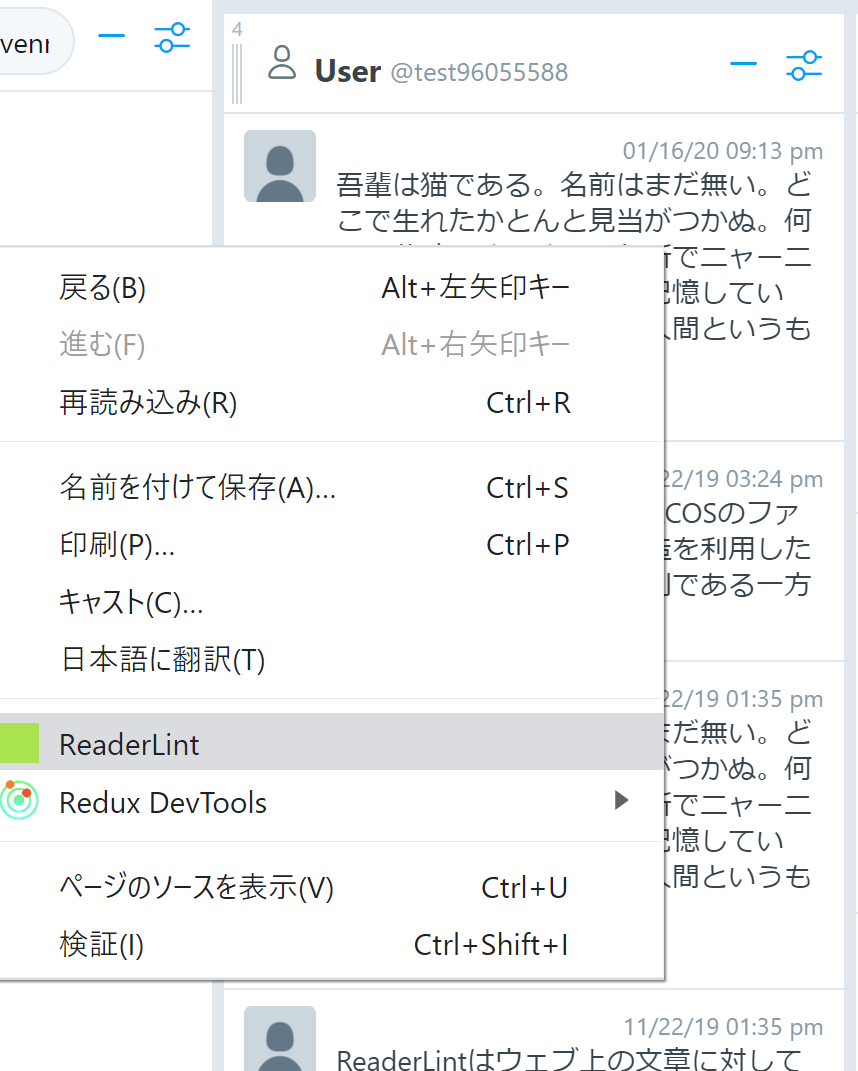
\includegraphics[width=0.6\columnwidth]{image/03/img0.png}
    \caption[コンテキストメニュー] {コンテキストメニュー}
\end{figure}
\begin{figure}[H]
    \centering
    \label{fig:image10}
    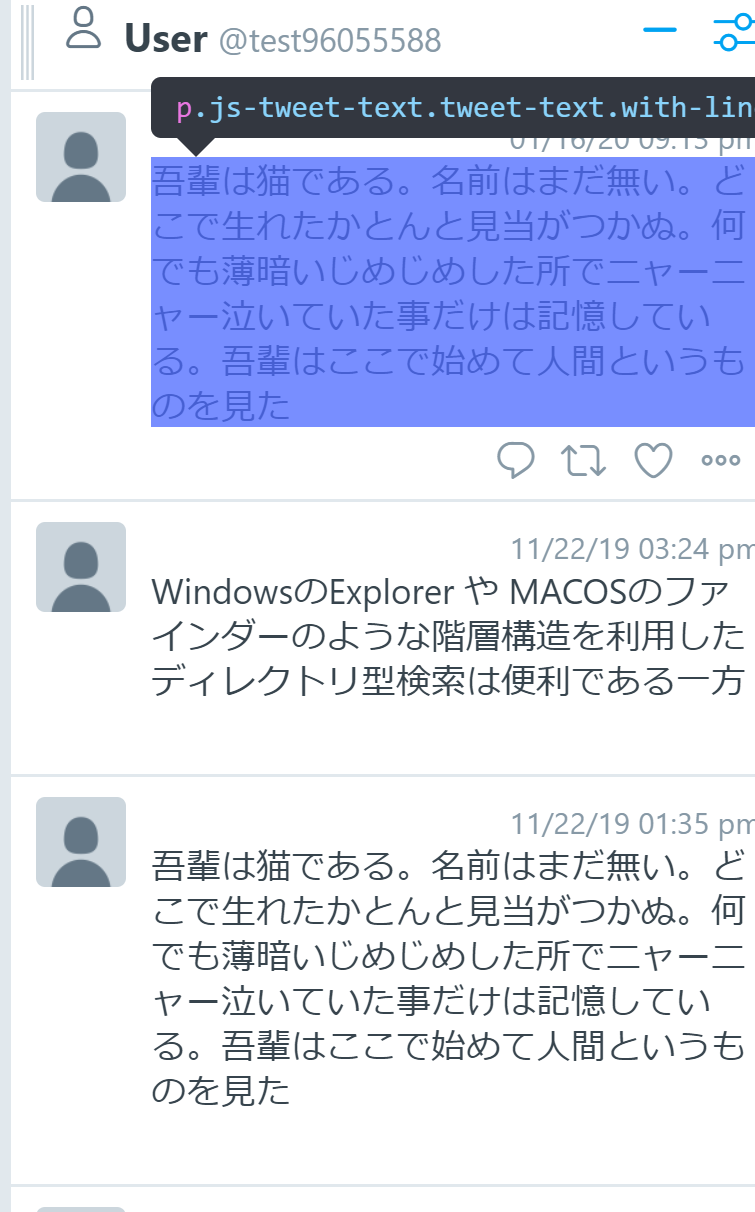
\includegraphics[width=0.6\columnwidth]{image/03/img1.png}
    \caption[DOM選択モード] {DOM選択モード}
\end{figure}

\begin{figure}[H]
    \centering
    \label{fig:image11}
    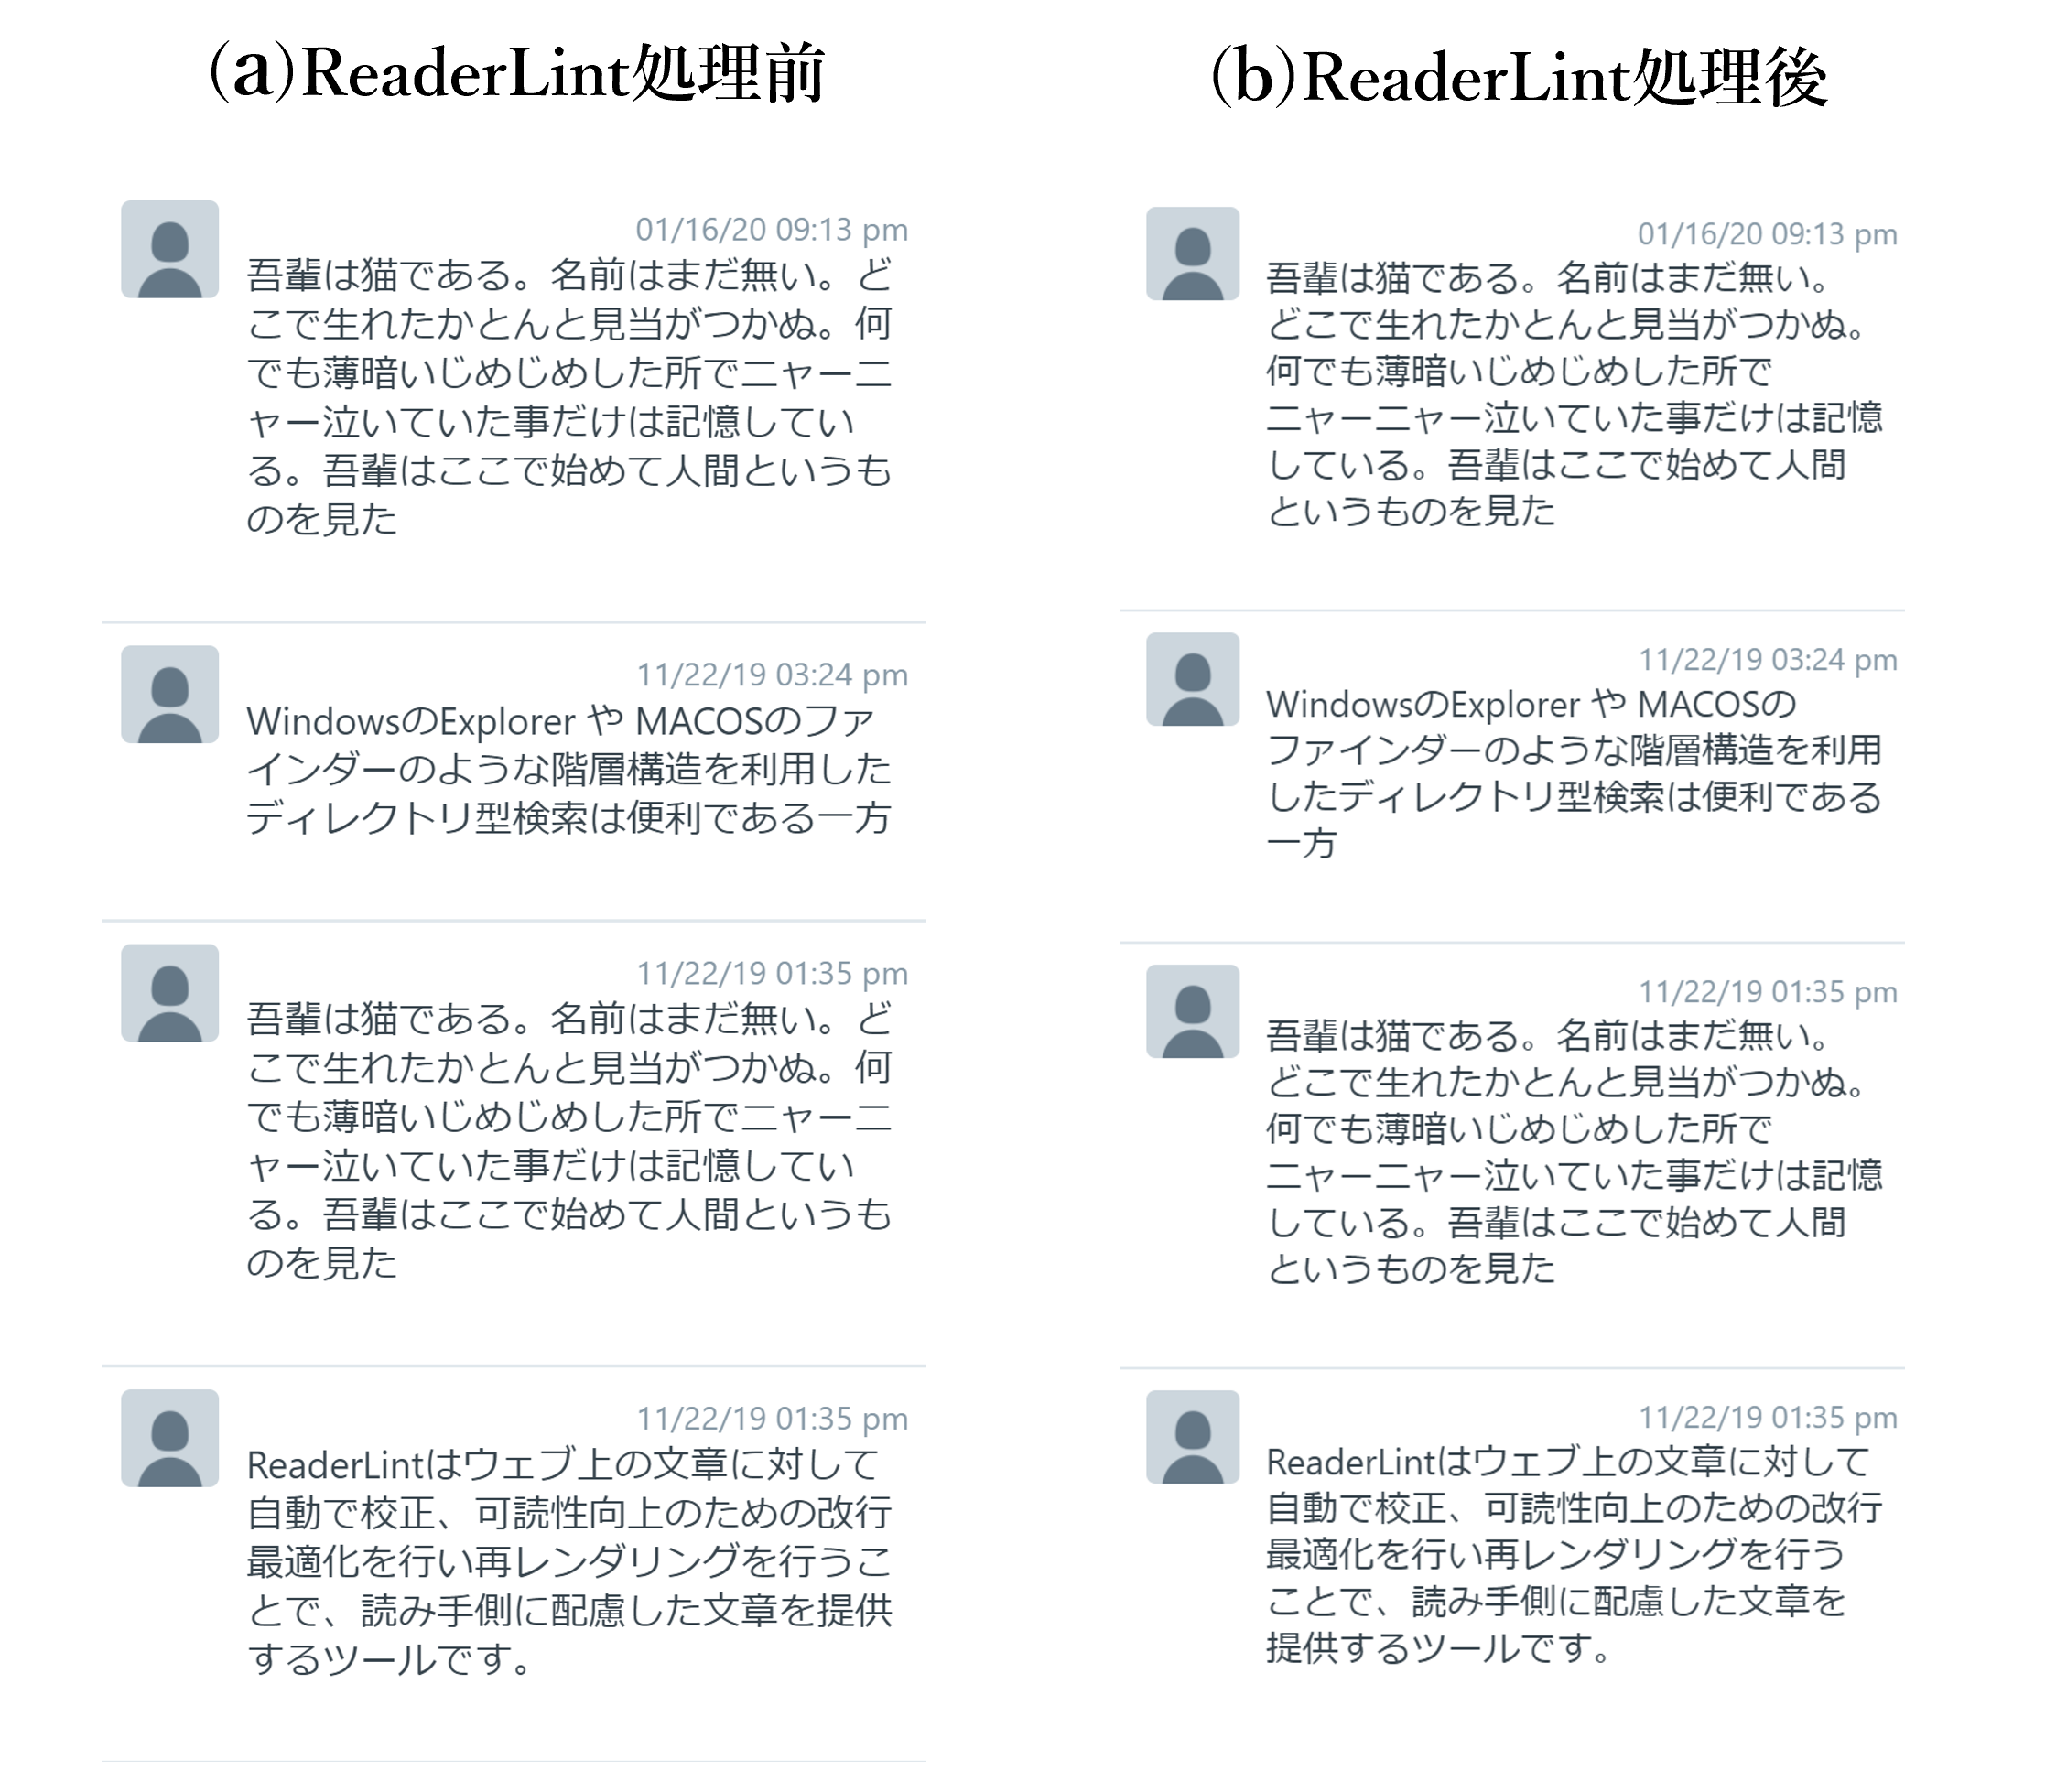
\includegraphics[width=0.6\columnwidth]{image/03/img2.png}
    \caption[文章の再形成が行われた画面]{文章の再形成が行われた画面}
\end{figure}

また、視認性の理由から文章の格納されているDOMのサイズが900pxを超えている場合には、
900pxに収まるよう調整をかけている。以下の画像は横幅が1345pxであった
DOMの文章にReaderLintを実行した際の動作である。\footnotemark[1]

\footnotetext[1]{参考: 
	\protect\url {https://anond.hatelabo.jp/20200112130927}
}

\begin{figure}[H]
    \centering
    \label{fig:image12}
    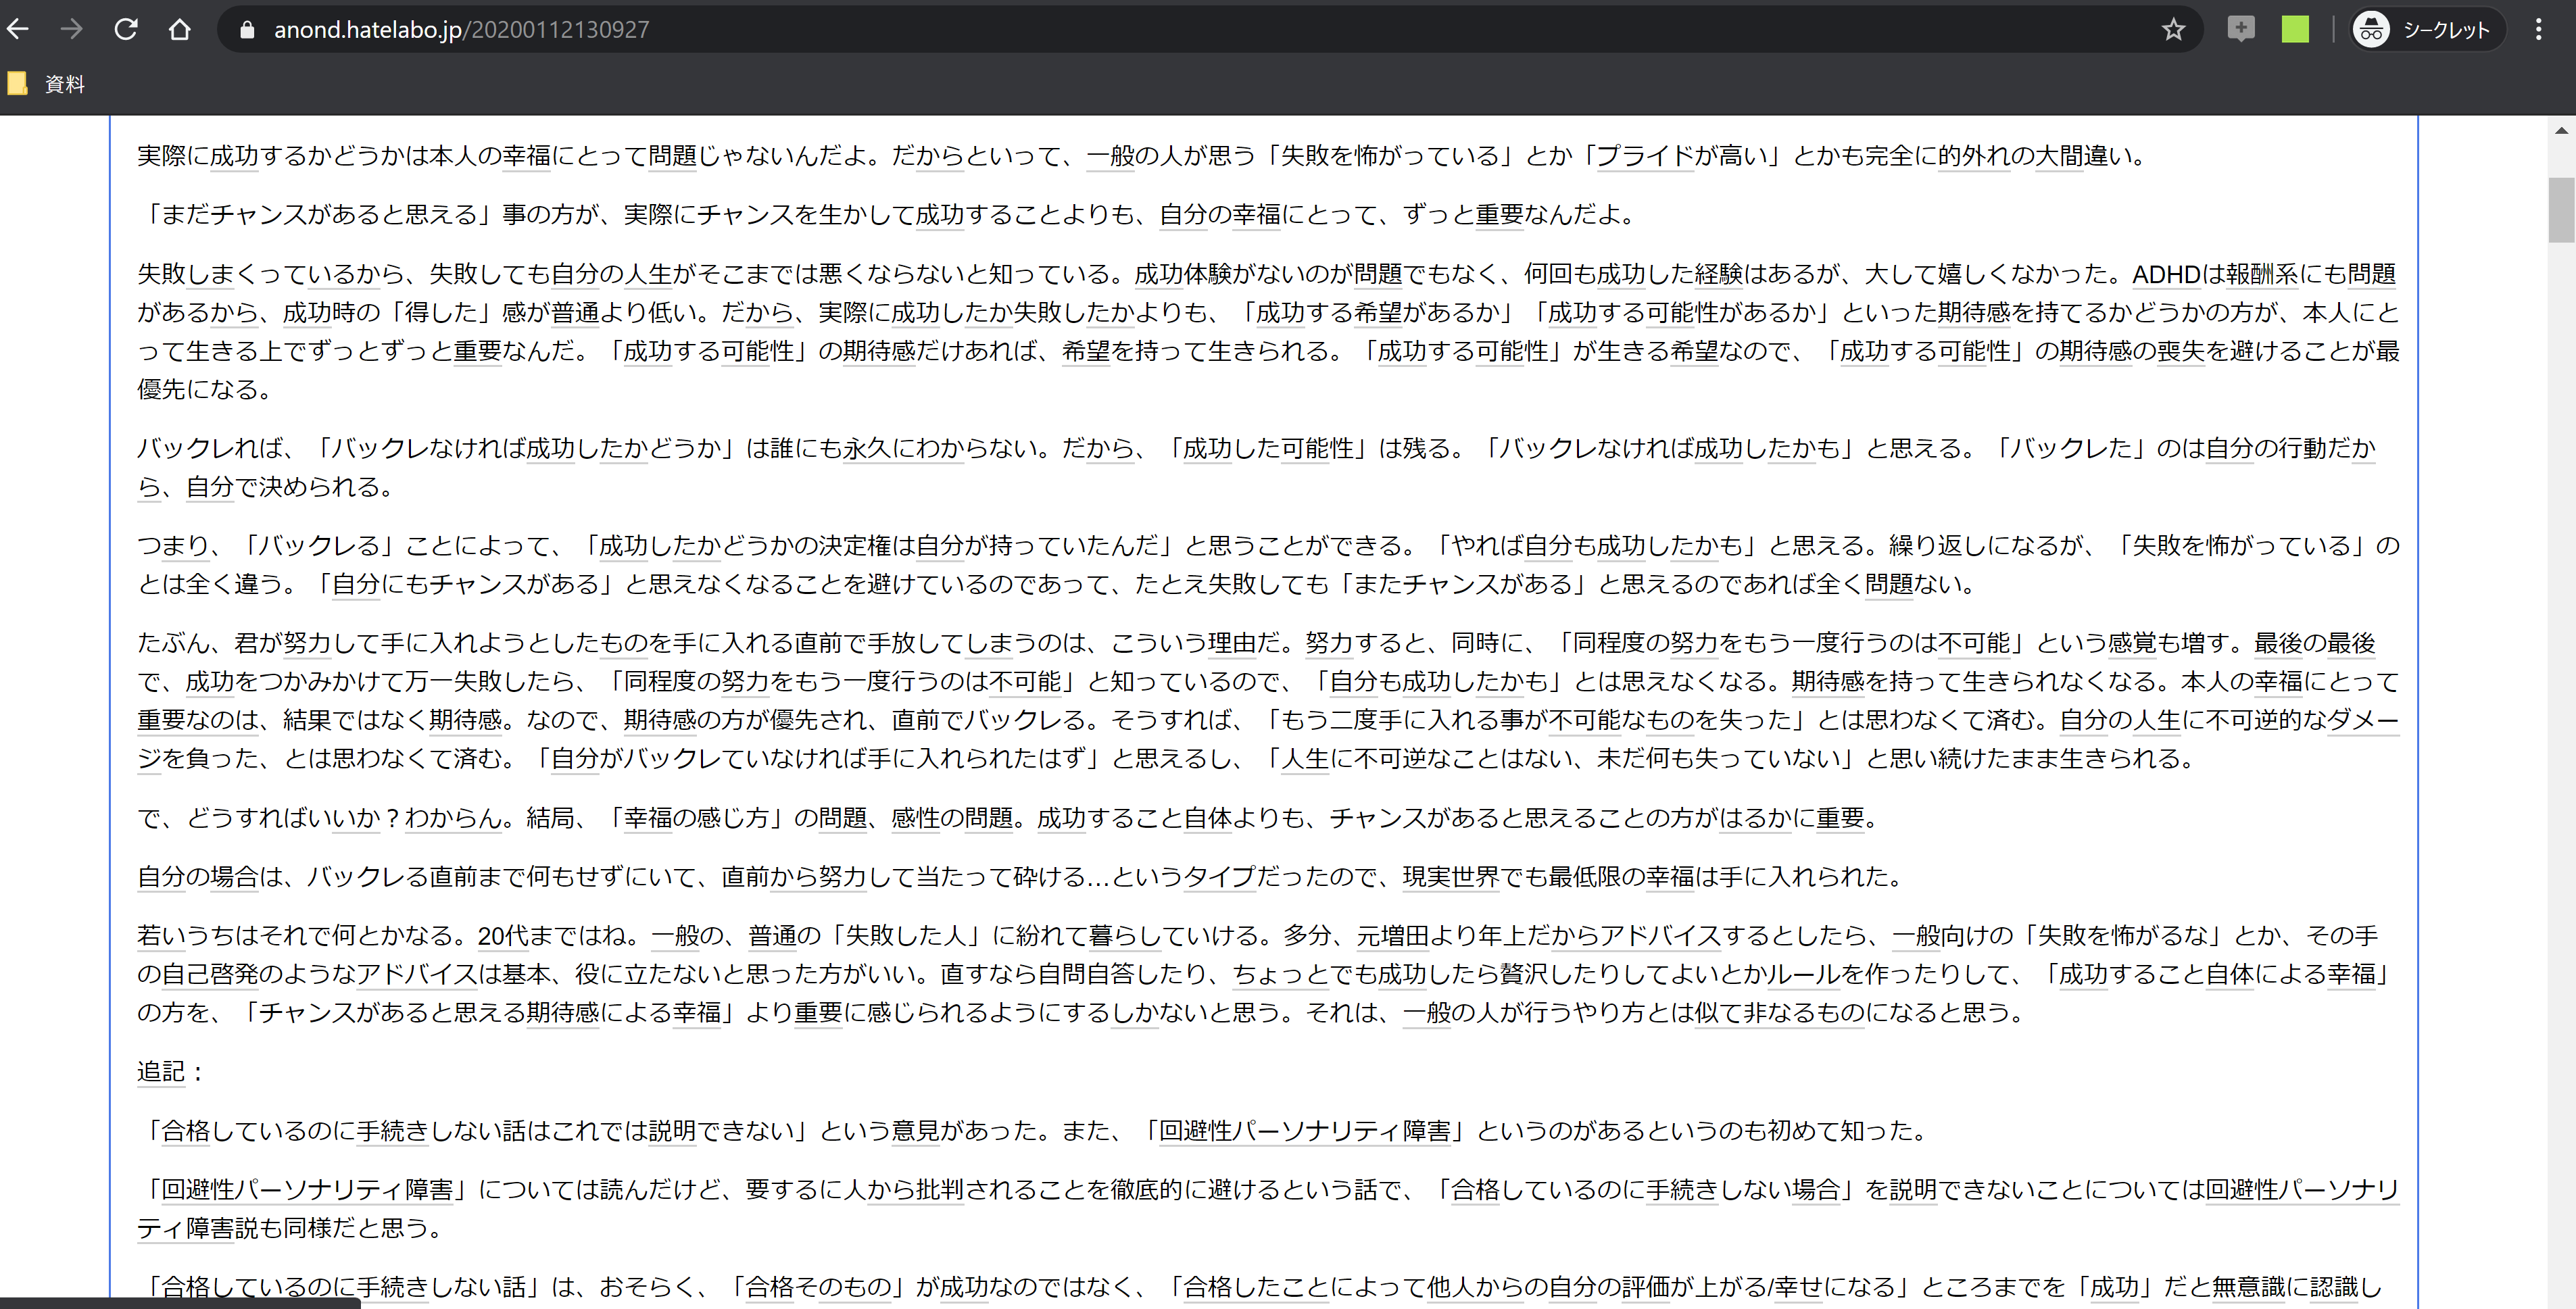
\includegraphics[width=0.8\columnwidth]{image/03/img3.png}
    \caption[横幅に調整をかける前]{横幅に調整をかける前}
\end{figure}
\begin{figure}[H]
    \centering
    \label{fig:image13}
    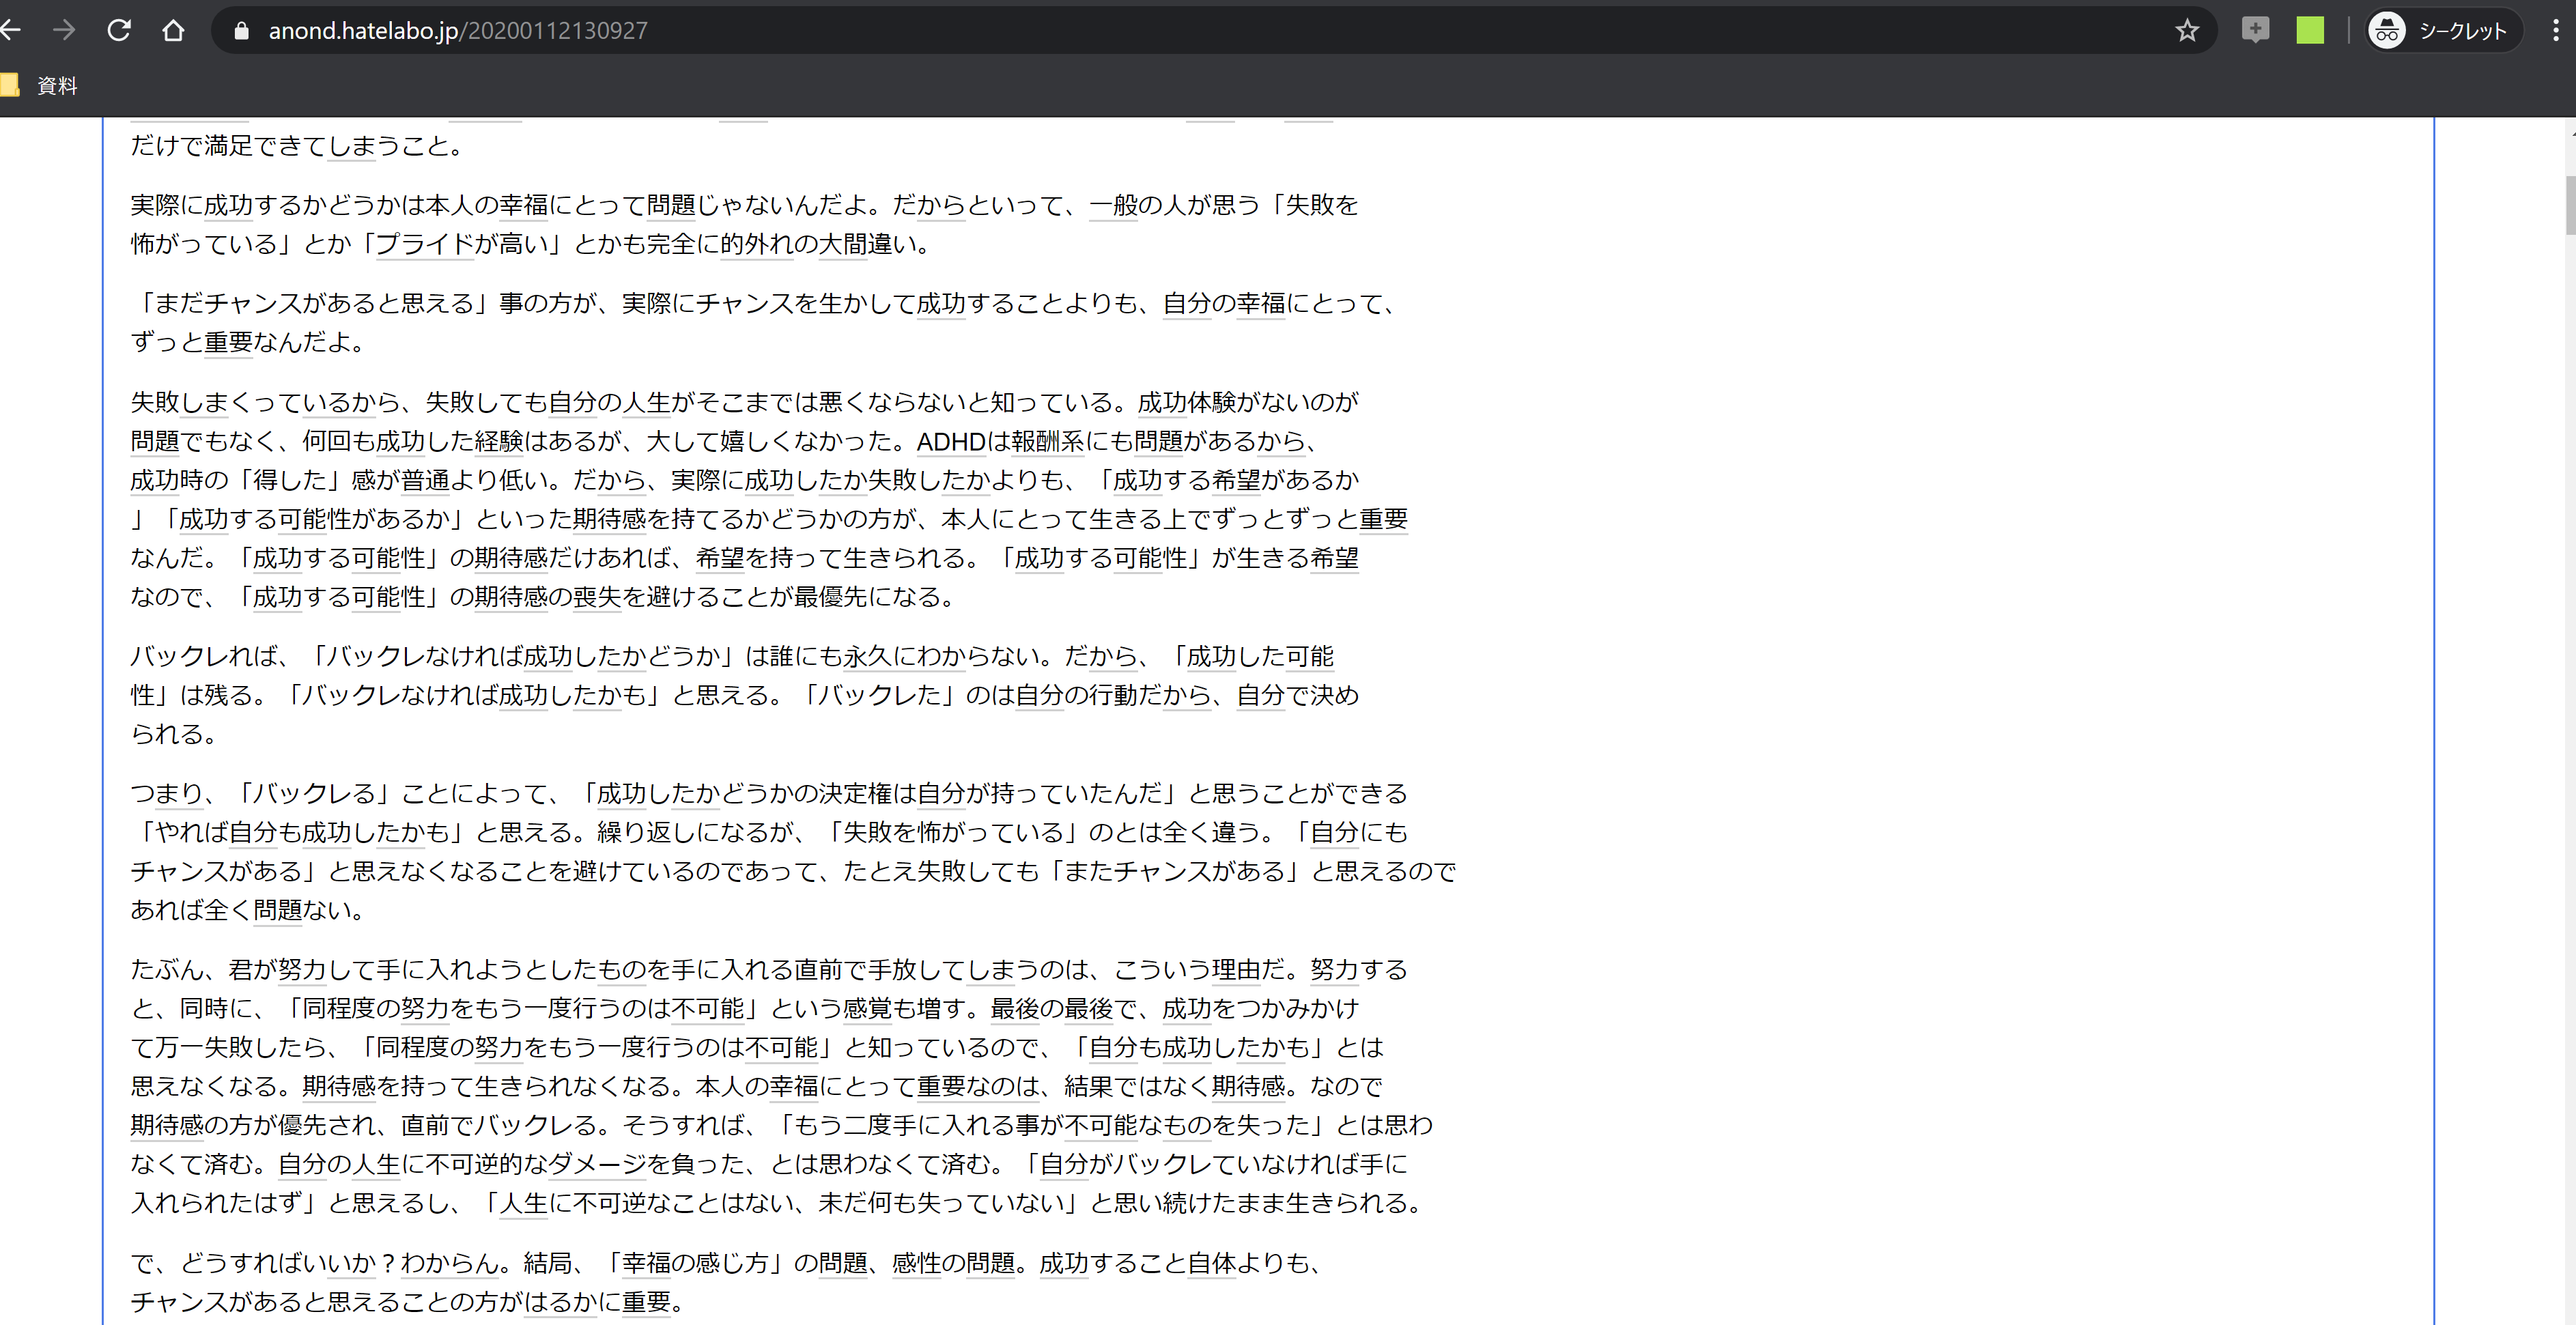
\includegraphics[width=0.8\columnwidth]{image/03/img4.png}
    \caption[横幅に調整をかけた後]{横幅に調整をかけた後}
\end{figure}

\section{実装}


\subsection{Domの取得}
ReaderLintを実行するDOMの取得にはDocument


\subsection{文章の折返し箇所の自動検出}
文節ごとに区切られた改行を行うためには、左詰された文章が指定したDOMの横幅(width)を超えるタイミング、
文章の折返し箇所を検知する必要がある。現在のWebAPIには日本語の文章を折り返す文字の箇所を自動検知できる機能は存在しない。
そのため、一度文章全体に文節ごとに分かち書きを行い、分かれた文節の横幅を計測し、順に配列として格納する。一行に含まれる文節ごとの描画幅の総和がDOMサイズを超過した際に、
その文節の前に改行文字を挿入し配列に加える、という検知方法を採用した。最後に完成した配列を連結させ、文字列として元のDOMのInnerHTMLに返すことで処理を加えたテキストを反映させた。

\begin{figure}[H]
    \centering
    \label{fig:image14}
    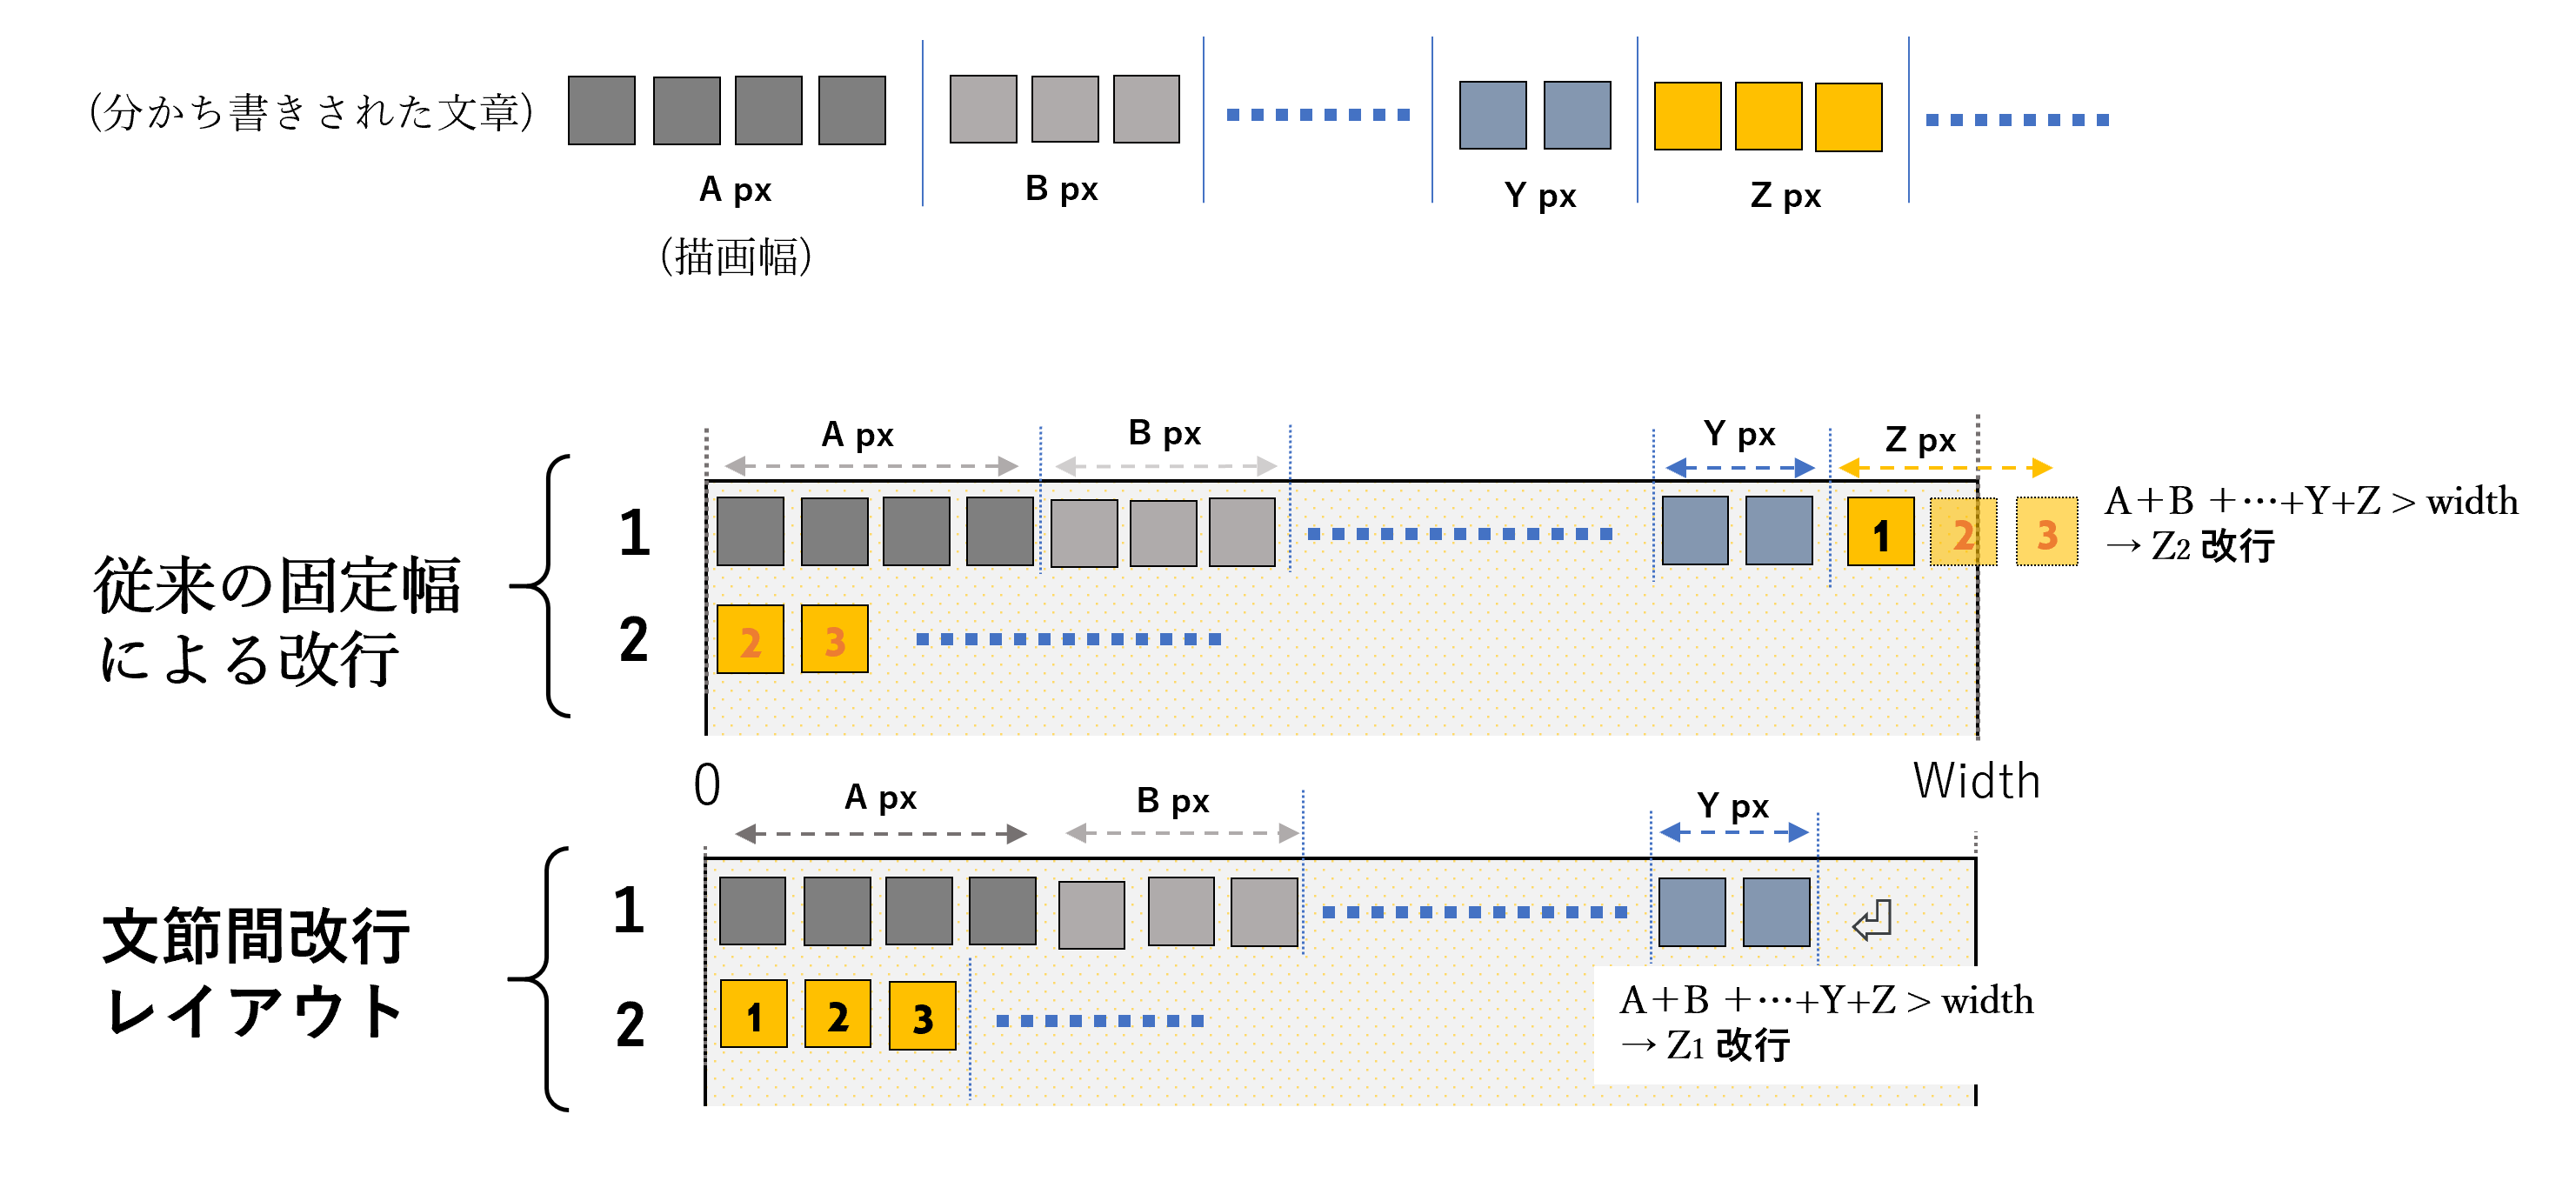
\includegraphics[width=0.8\columnwidth]{image/03/img6.png}
	\caption[文節ごとの改行処理]{文節ごとの改行処理]}
\end{figure}

この方法を実装するには日本語の分かち書きにより文節ごとに分けること、および各文節の文字幅の予測が必要となる。
この処理を行なうために用いた方法として以下の二つを紹介する

\subsubsection{日本語分かち書き}
文章に対して文節ごとに区切る分かち書きの、文章を文節ごとに区切る、といった日本語分かち書きを行うライブラリには
辞書ベースのデータに頼る辞書あり型と、大まかな解析データに頼る辞書なし型の二つに大別される。
\\今回は辞書なし型であるtinySegmenterを用いた。tinySegmenterとは工藤匠氏が開発し、
公開しているJavaScript製の日本語分かち書きライブラリである。\footnotemark[2]
TinySegmenterには以下の特色がある。

\begin{enumerate}
	\item 25キロバイトという軽量さ
	\item JavaScript製であり、クライアントサイドに組み込むだけで分かち書き処理が可能
	\item 機械学習のみで辞書データに非依存的である故に、辞書のロード時間がなく、高速である点
	\item くだけた文章表現には弱い一方、辞書に登録されていない未知語に対して検出率が高い点
\end{enumerate}
辞書型よりも分かち書きの精度は低くなるが、上記の利点を加味して使用する。

\footnotetext[2]{
	参照: \protect\url {http://chasen.org/~taku/software/TinySegmenter/}
}

\subsubsection{canvas.context.measureTextメソッドを用いた文字幅の計測}
canvasとはHTML5にて追加されたHTML上にてビッドマップキャンバスを用いた視覚的な画像をレンダリングすることを目的とした
HTML要素である。canvasが提供する機能のうち2DコンテキストAPIのmeasureTextはcanvas上でレンダリングしたテキストの描画幅を測定し、
ピクセル単位で返してくれるメソッドである。描画幅として計測されるのは指定したフォントでテキストを描画した場合の描画幅であるため、
文章を格納しているDOMのフォント設定とフォントサイズを設定すれば、DOMにてレンダリングされている文字幅の数値のシミュレートが可能となる。
\\上記の二つを用いて文章サイズを計測することで文章の折返し箇所の自動検出を実装した。

\subsection{ASTを用いた文章解析}
DOMの内部にはリンク、画像、改行といった文字列以外の処理が存在するため、
あらかじめ文章の種類を分別し、その種類ごとに処理を行う必要がある。
文章の種類を分別する手法として、今回はAST(抽象木構造,Abstract Syntax Tree)を用いる。
\\ASTとしてあらかじめ種類を分けておくことで、加える処理を分けておく
今回は文章に対して抽象構文木(Abstract Syntax Tree,以下AST)を用いて処理を行う。
ASTとは本来はプログラミング言語の静的解析やそれに基づいた処理を行う際に、
用いられる文字列をデータ構造である。
\begin{figure}[H]
    \centering
    \label{fig:image15}
    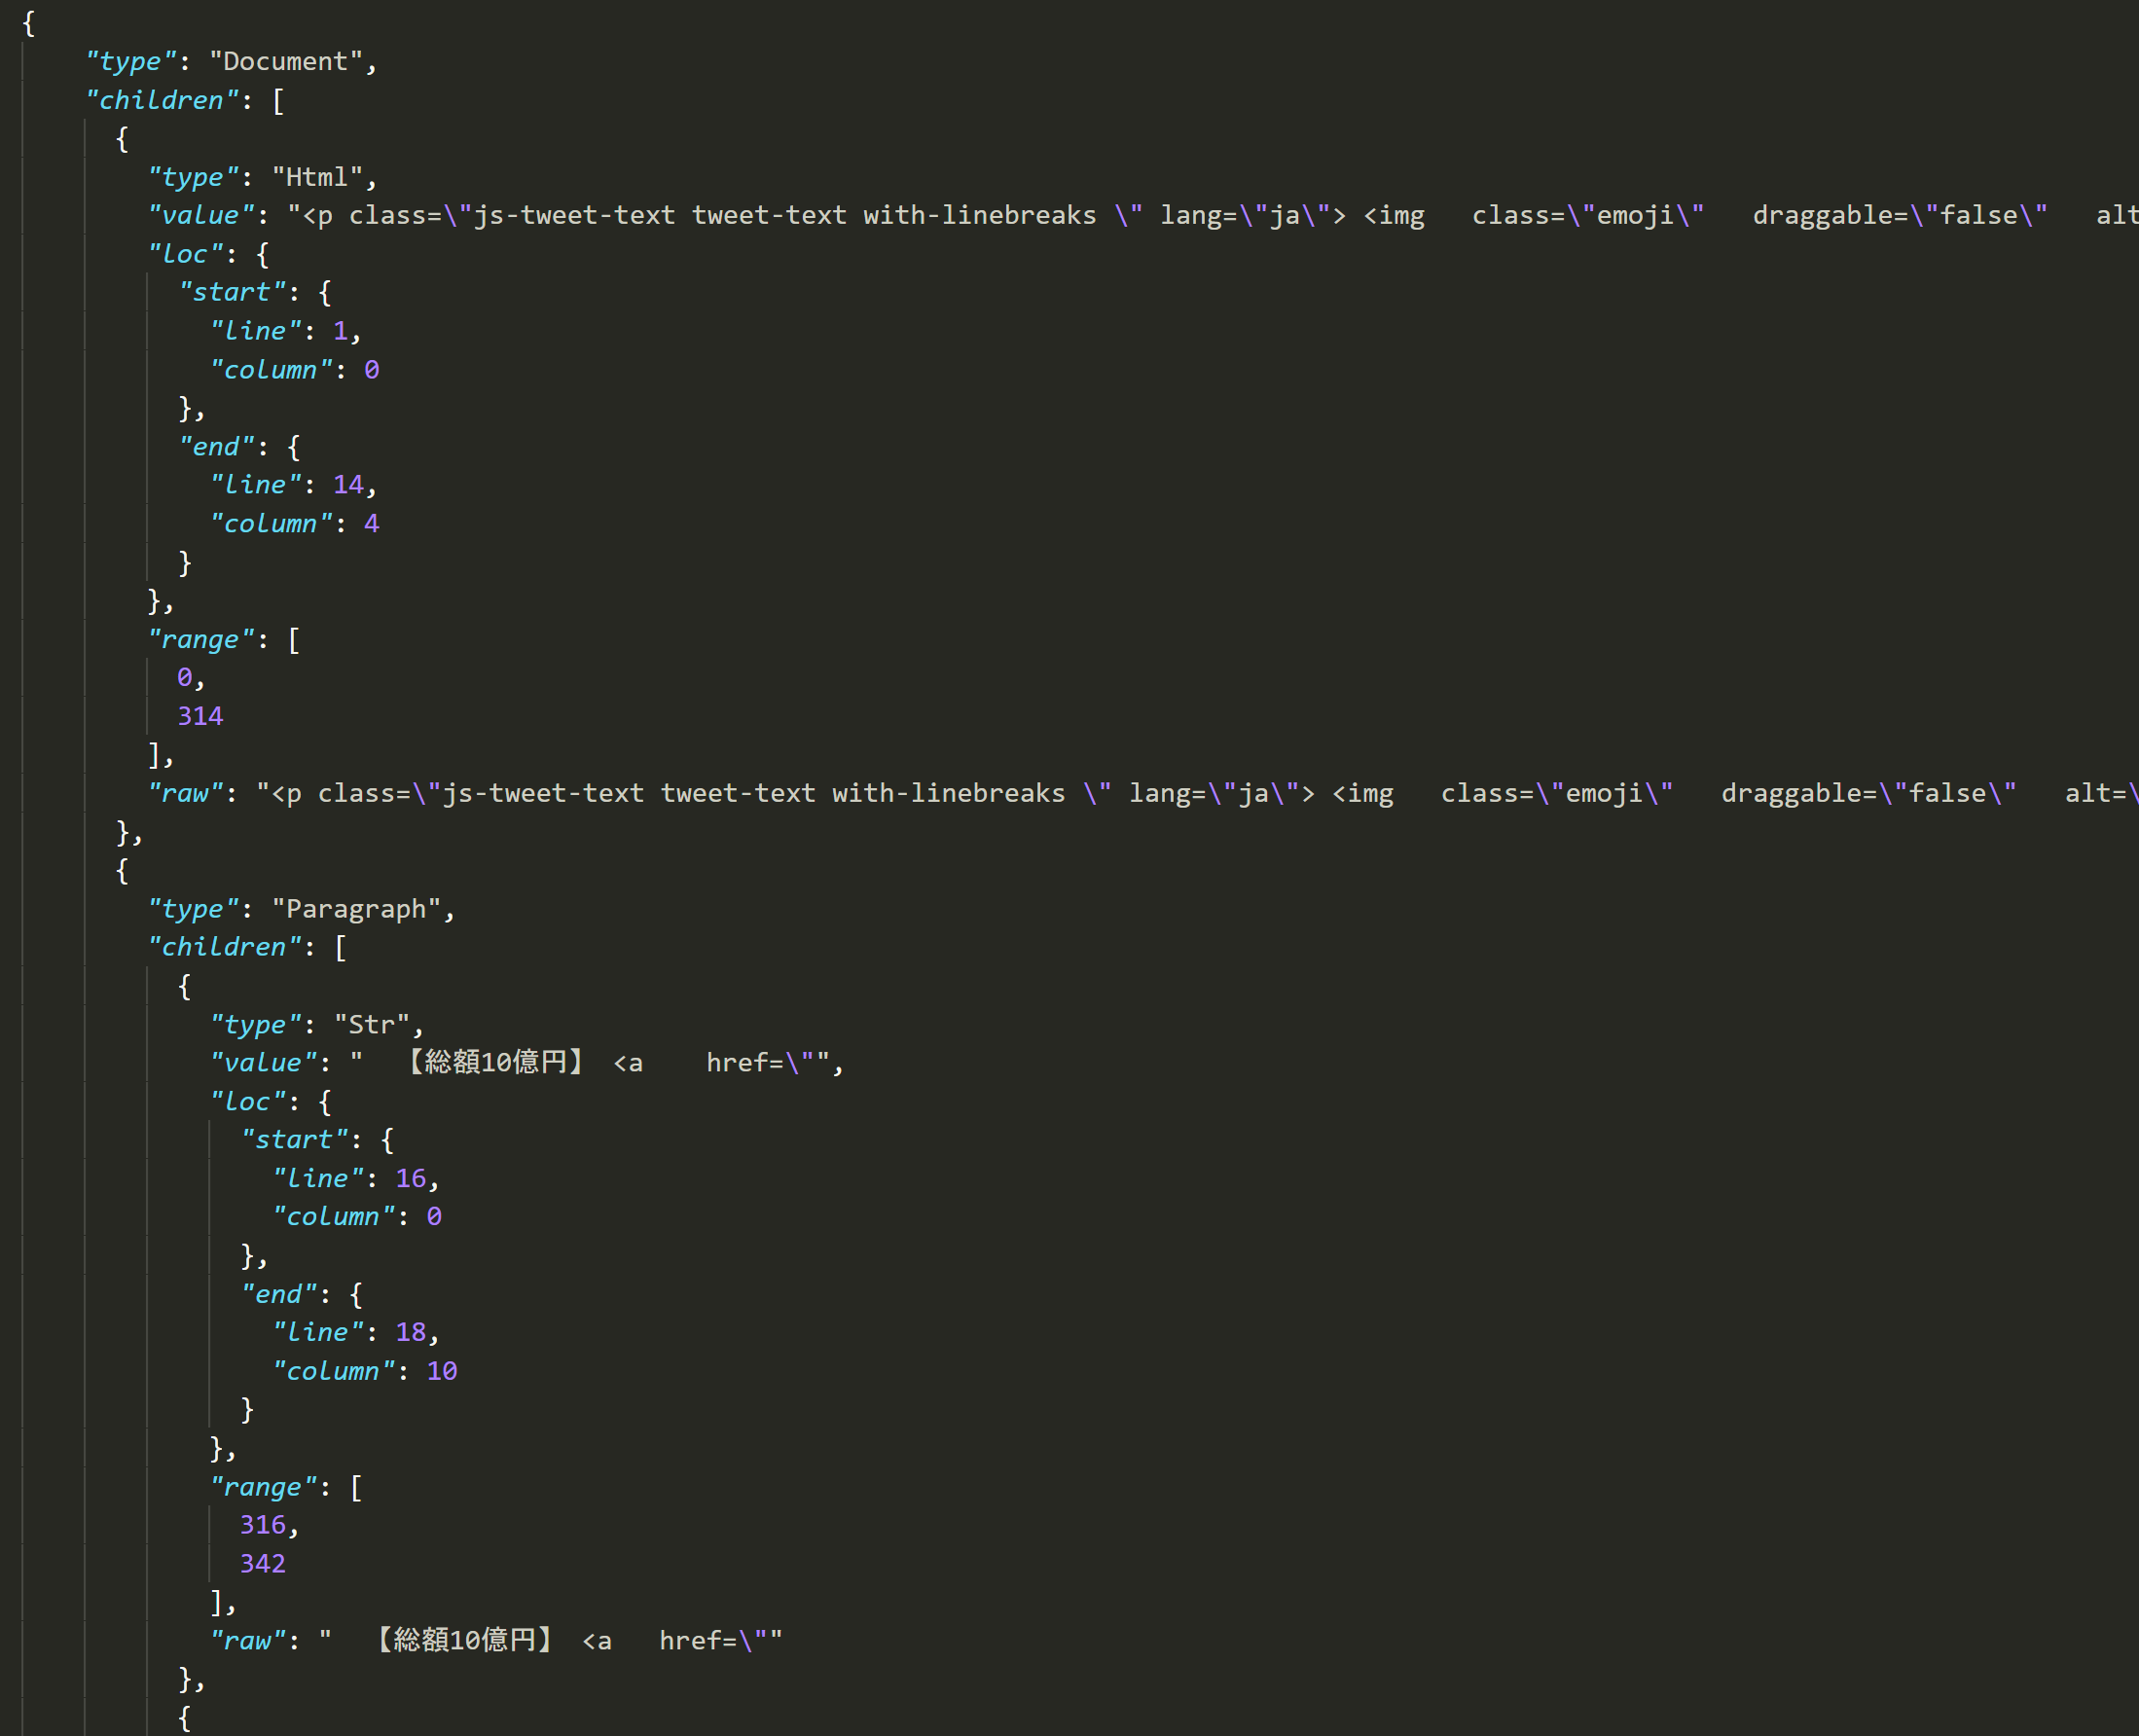
\includegraphics[width=0.8\columnwidth]{image/03/img5.png}
	\caption[テキストをAST化し見やすくした図]{テキストをAST化し見やすくした図}
\end{figure}

今回利用したASTライブラリは、実際に文章としてレンダリングされた箇所と、DOM内で記述されるHTMLタグの内容とを分別して
ASTを出力するtextlint/markdown-to-astに改行箇所を示すエスケープシーケンス$\backslash$n
を検知する仕様に変更したものと\footnotemark[2]、AST化した文章の種類ごとにその文字列に施す処理を記述できるtextlint/ast-to-traverseを使用する。\footnotemark[3]
\footnotetext[2]{参考: 
	\protect\url {https://github.com/textlint/textlint/tree/master/packages/@textlint/markdown-to-ast}
}
\footnotetext[3]{参考: 
	\protect\url {https://github.com/textlint/textlint/tree/master/packages/@textlint/ast-traverse}
}

ASTによって文章を識別する利点は、ブラウザ上にレンダリングされているリンクやハッシュタグ、といったHTML要素に由来する表記を非破壊的に監査できる点にある。
HTMLタグの中身である文章としてレンダリングされている箇所だけを文節として取り出し、加算処理を行なった上で配列にHTMLごとを格納することで、
挿入されたHTMLタグ全体の文字幅を計測やタグ内中の文字列に改行コードを入れてしまい、HTML要素を破壊してしまうことを防ぐことができる。
\begin{figure}[H]
    \centering
    \label{fig:image16}
    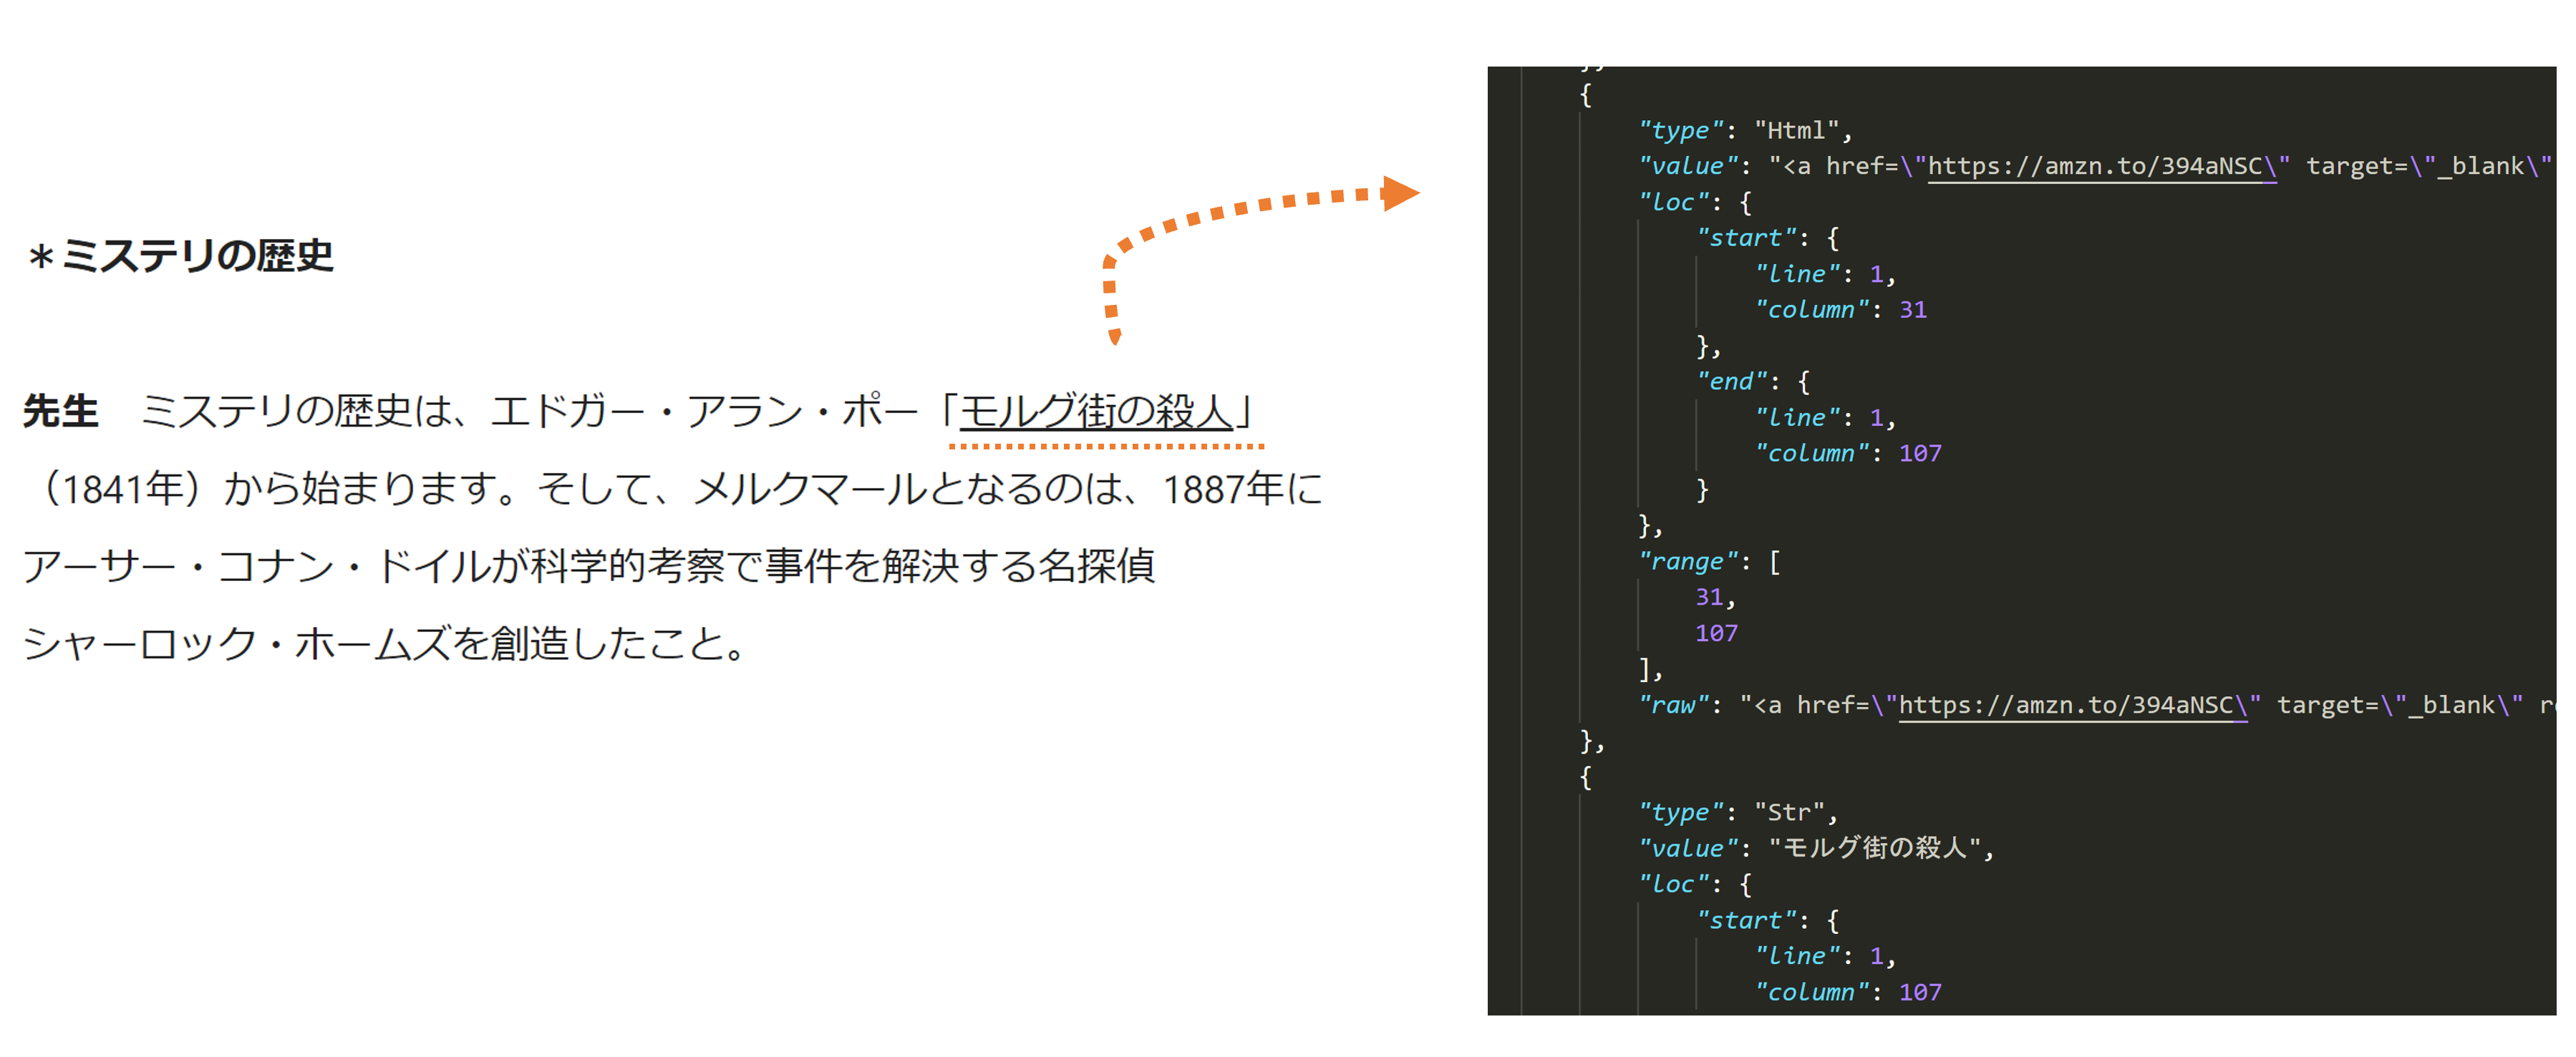
\includegraphics[width=0.8\columnwidth]{image/03/img7.png}
	\caption[HTMLタグ内の文章を分けて処理する図]{HTMLタグ内の文章を分けて処理する図} \footnotemark[4]
\end{figure}

\footnotetext[4]{使用サイト参照:
	\protect\url{https://www.hayakawabooks.com/n/ncdfb31dc4e46?creator_urlname=hayakawashobo01}
}




